\documentclass[journal, a4paper]{IEEEtran}

\usepackage{graphicx}   

\usepackage{url}        

\usepackage{amsmath} 


% Your document starts here!
\begin{document}

% Define document title and author
	\title{Bitcoin Blockchain Visualization}
	\author{Zhiyi Xu, and Ruolan Zeng}
	\maketitle

% Write abstract here
\begin{abstract}

\end{abstract}
                                                   
% Each section begins with a \section{title} command
\section{Introduction}
	% \PARstart{}{} creates a tall first letter for this first paragraph
	\PARstart {B}{lockchain} and bitcoin are both hot topics these days. Bitcoin is a distributed, decentralized crypto-currency. A blockchain is a distributed database that is used to maintain a continuously growing list of records, called blocks. Bitcoin uses the blockchain protocol to serialize transactions of the bitcoin currency among its users. Figure 1 is an image briefly introducing how blockchain works for bitcoin.
\begin{figure}[!hbt]
		\begin{center}
		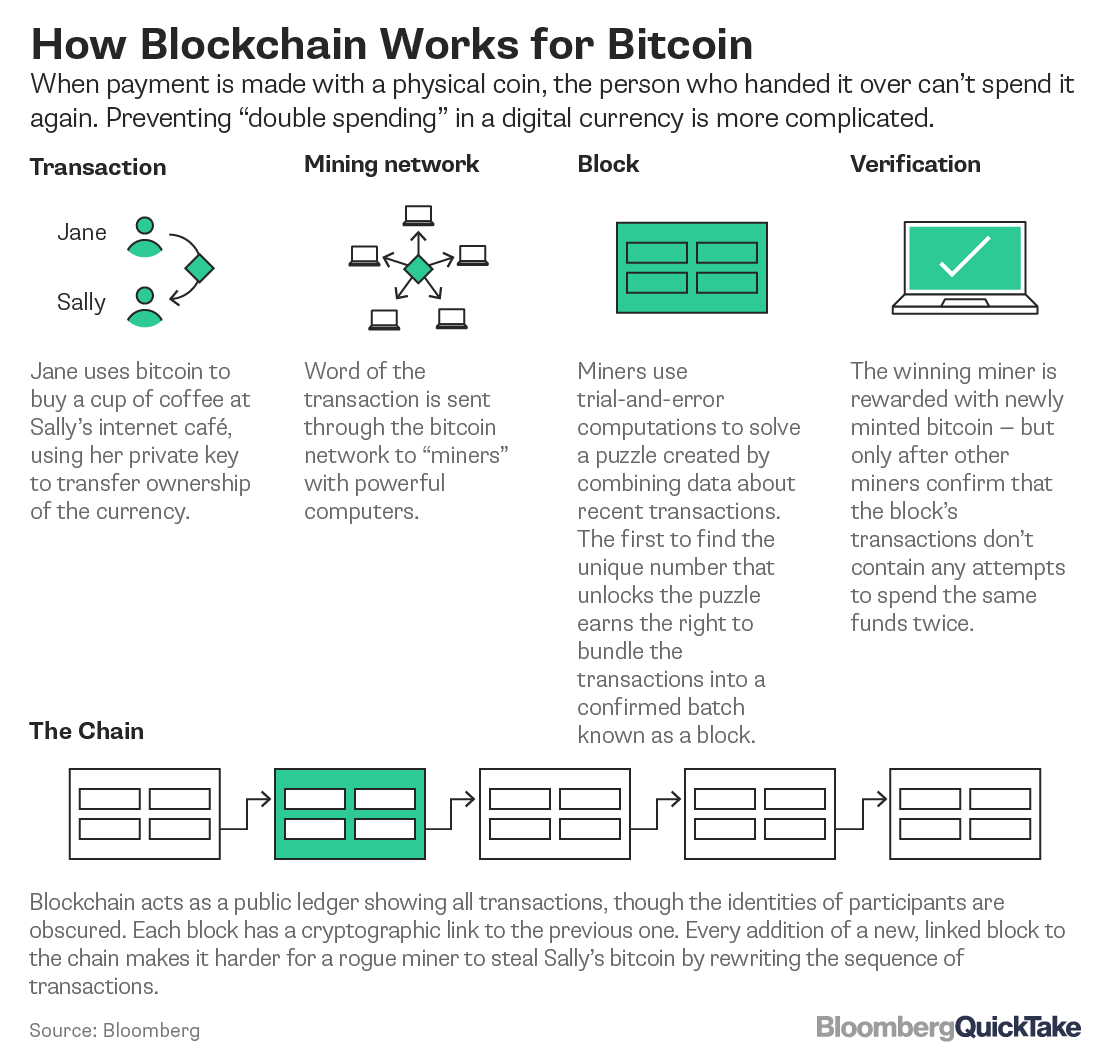
\includegraphics[width=\columnwidth]{how_blockchain_works.png}
		\caption{an image briefly introducing how blockchain works for bitcoin}
		\label{fig:how_blockchain_works}
		\end{center}
	\end{figure}

\section{Motivation}
This is a learning project during which we want to mock and visualize the bitcoin blockchain.

\section{Gap}

\section{Problem statement}

\section{Overall design}

\begin{figure}[!hbt]
		\begin{center}
		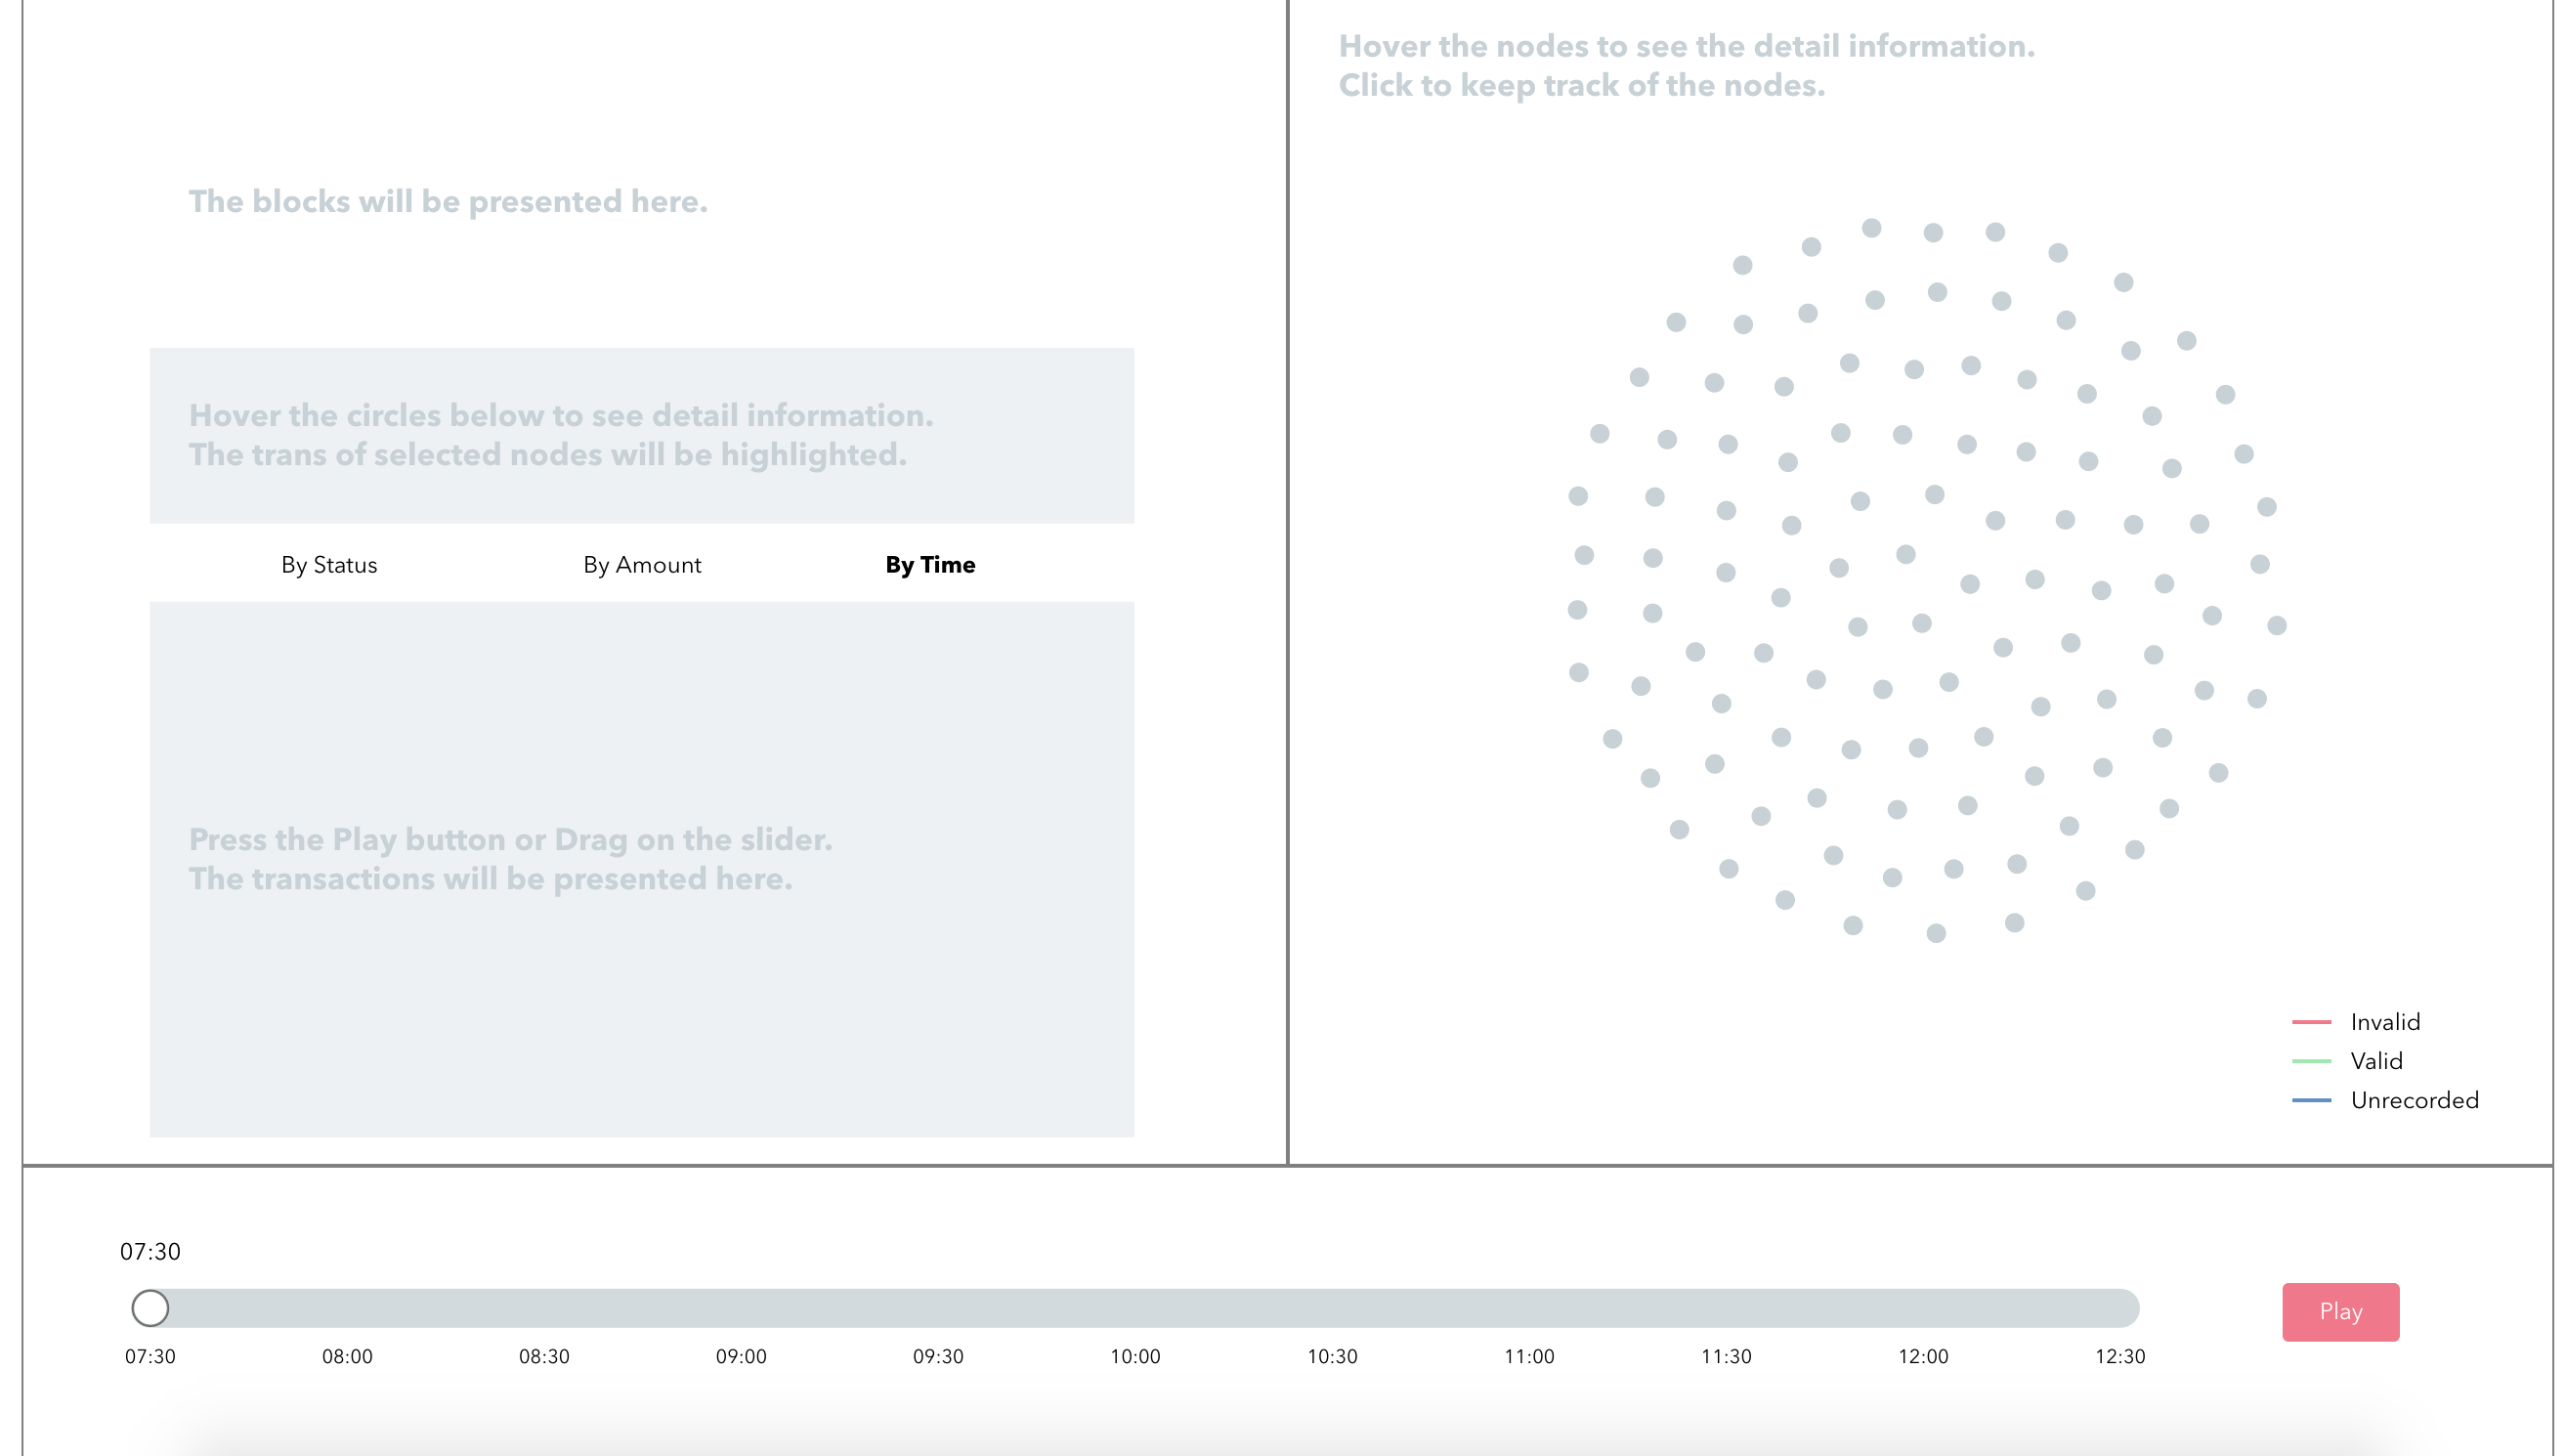
\includegraphics[width=\columnwidth]{overall_design_start.png}
		\caption{}
		\label{fig:overall_design}
		\end{center}
	\end{figure}

\begin{figure}[!hbt]
		\begin{center}
		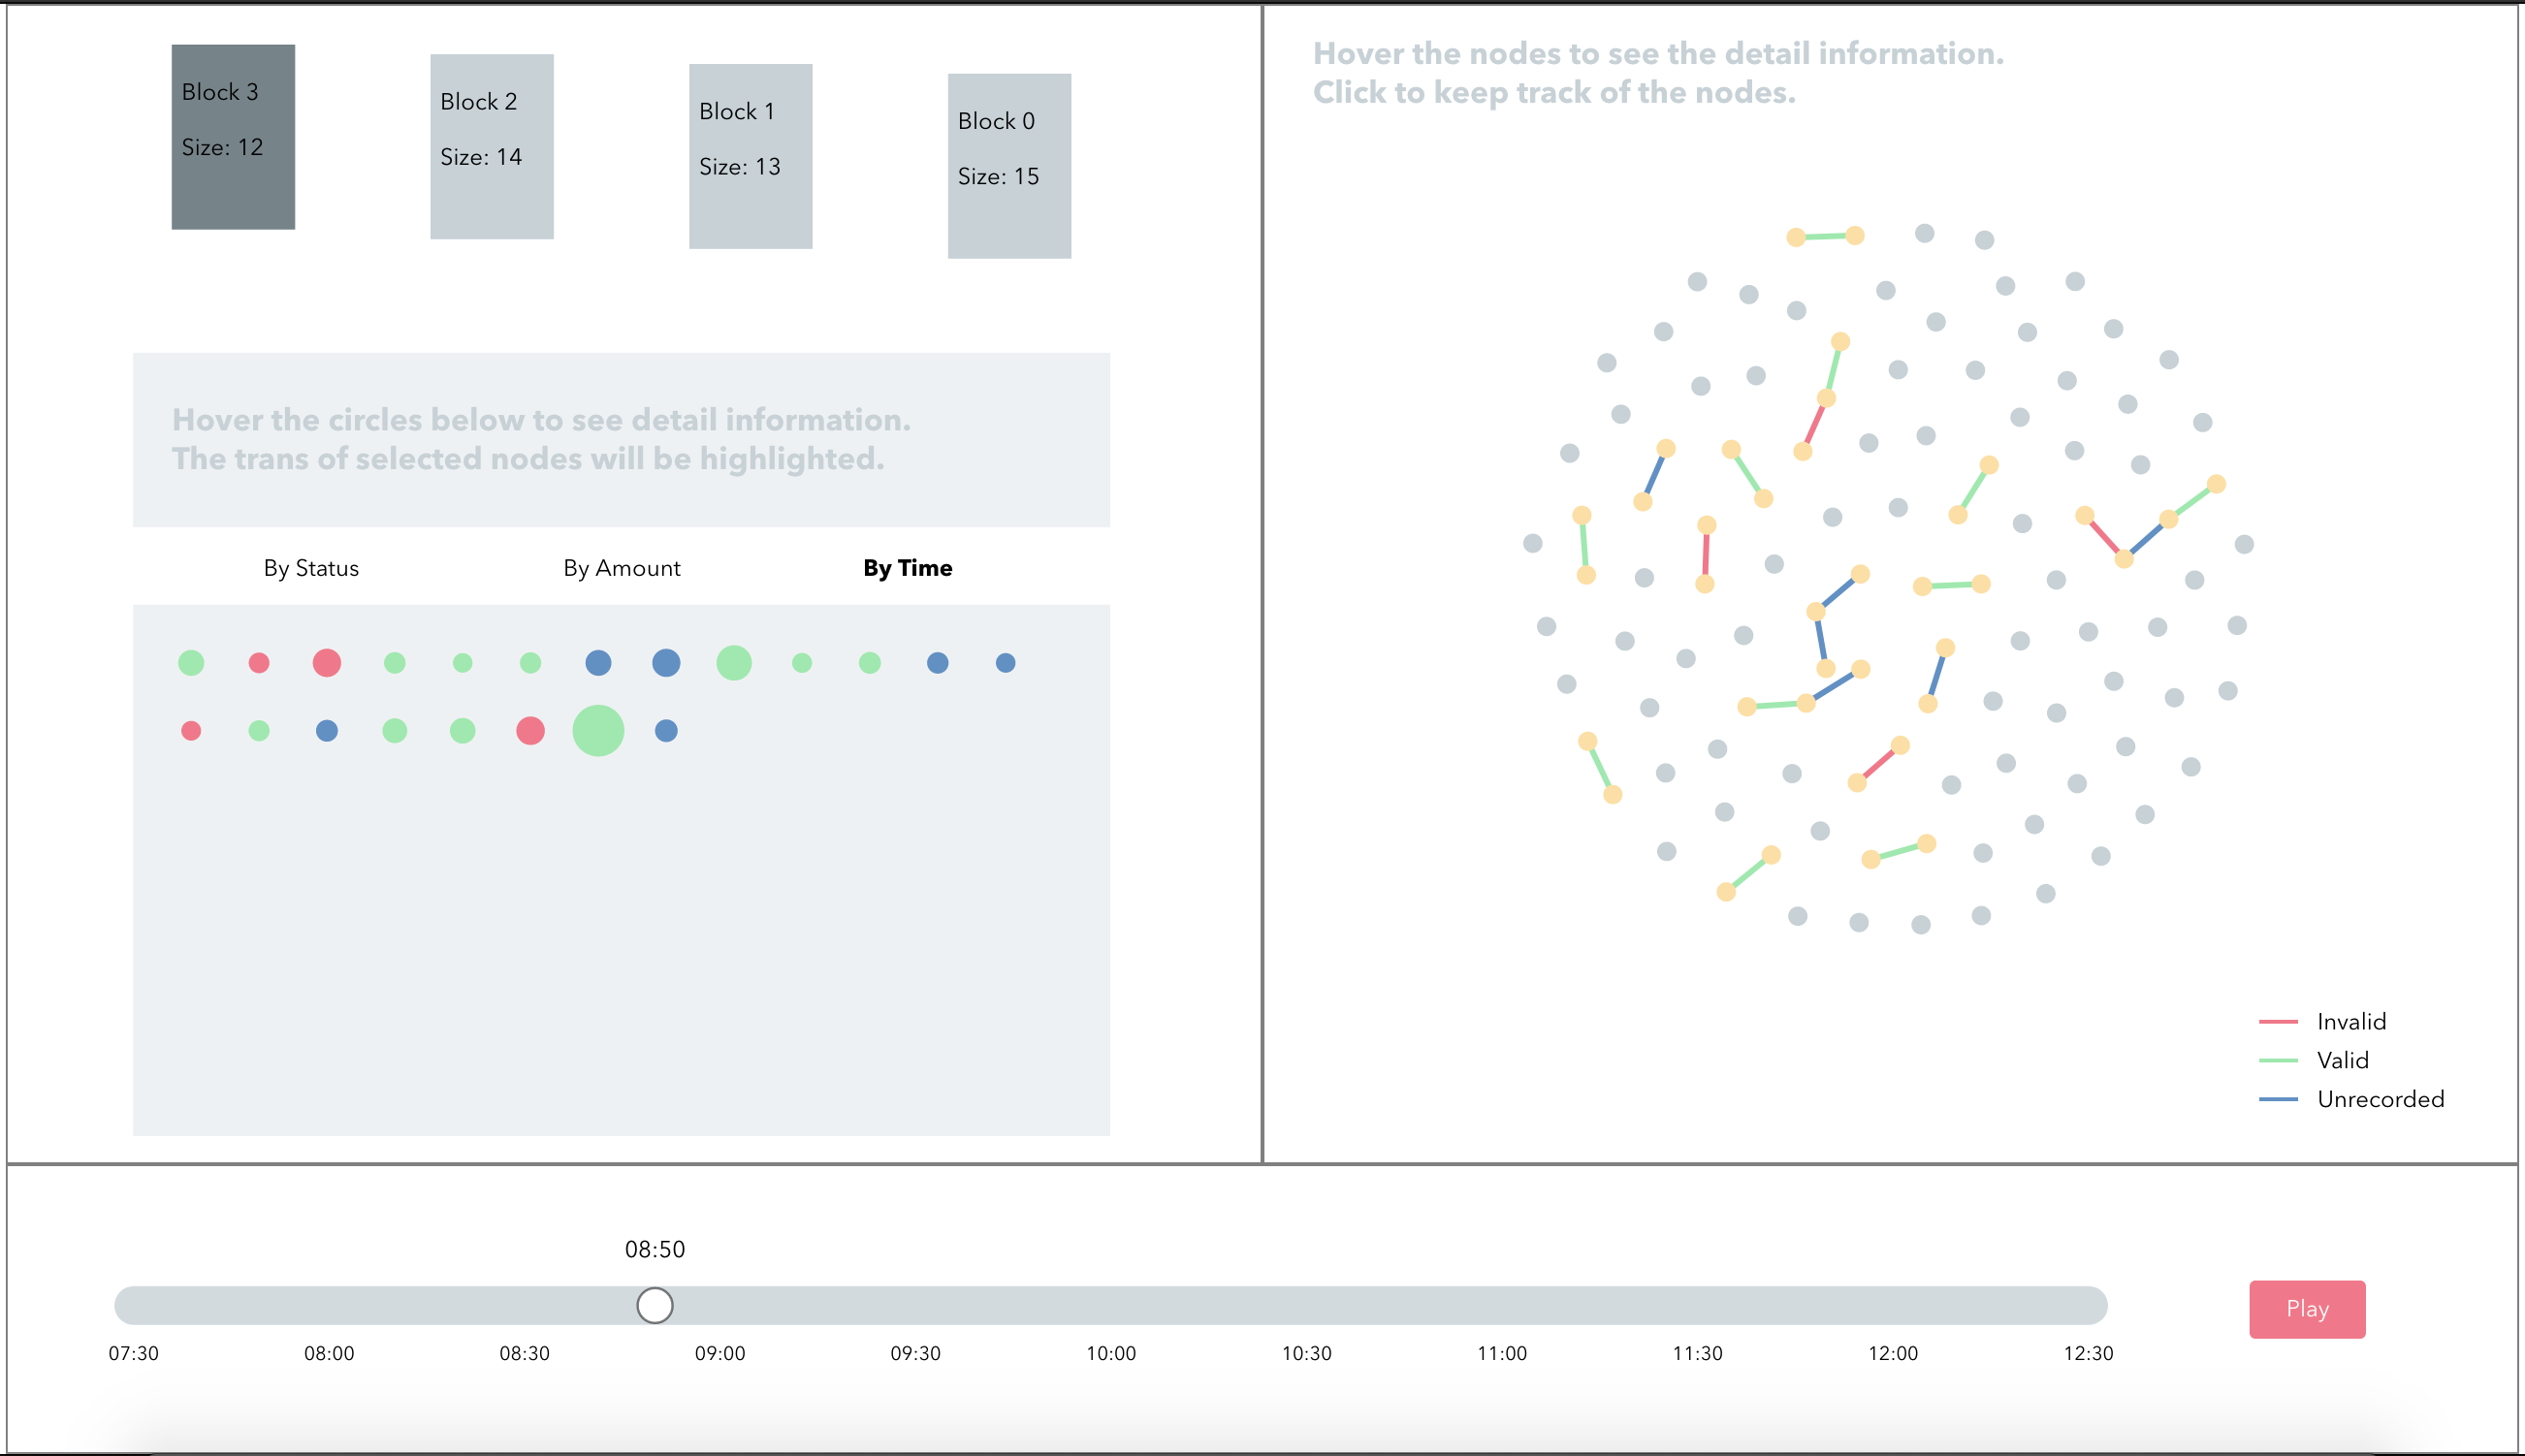
\includegraphics[width=\columnwidth]{overall_design.png}
		\caption{}
		\label{fig:overall_design}
		\end{center}
	\end{figure}
\section{Key intuitions behind our proposed design}
\subsection{Disjoint Force-Directed Graph}
\subsection{Blockchain Demo}
\subsection{Ethereum blockchain visualization}
\section{Key benefits of our proposed design}

\section{Details of our design}
\subsection{Transactions}

\begin{figure}[!hbt]
		\begin{center}
		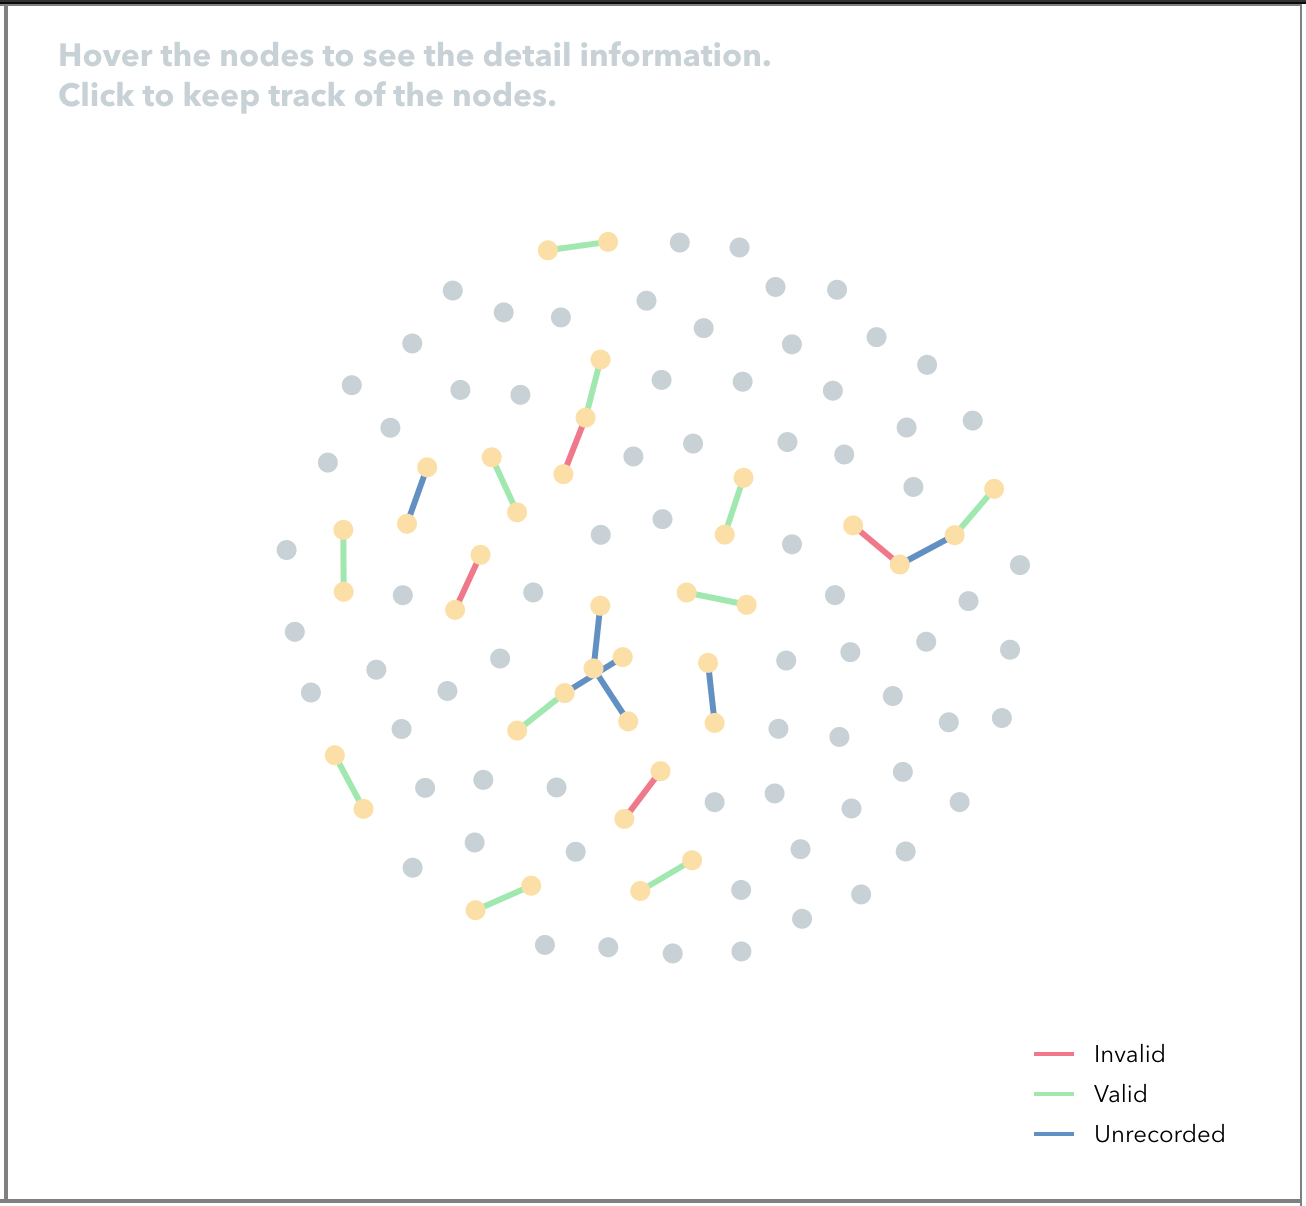
\includegraphics[width=\columnwidth]{transactions.png}
		\caption{}
		\label{fig:overall_design}
		\end{center}
	\end{figure}
	
\begin{figure}[!hbt]
		\begin{center}
		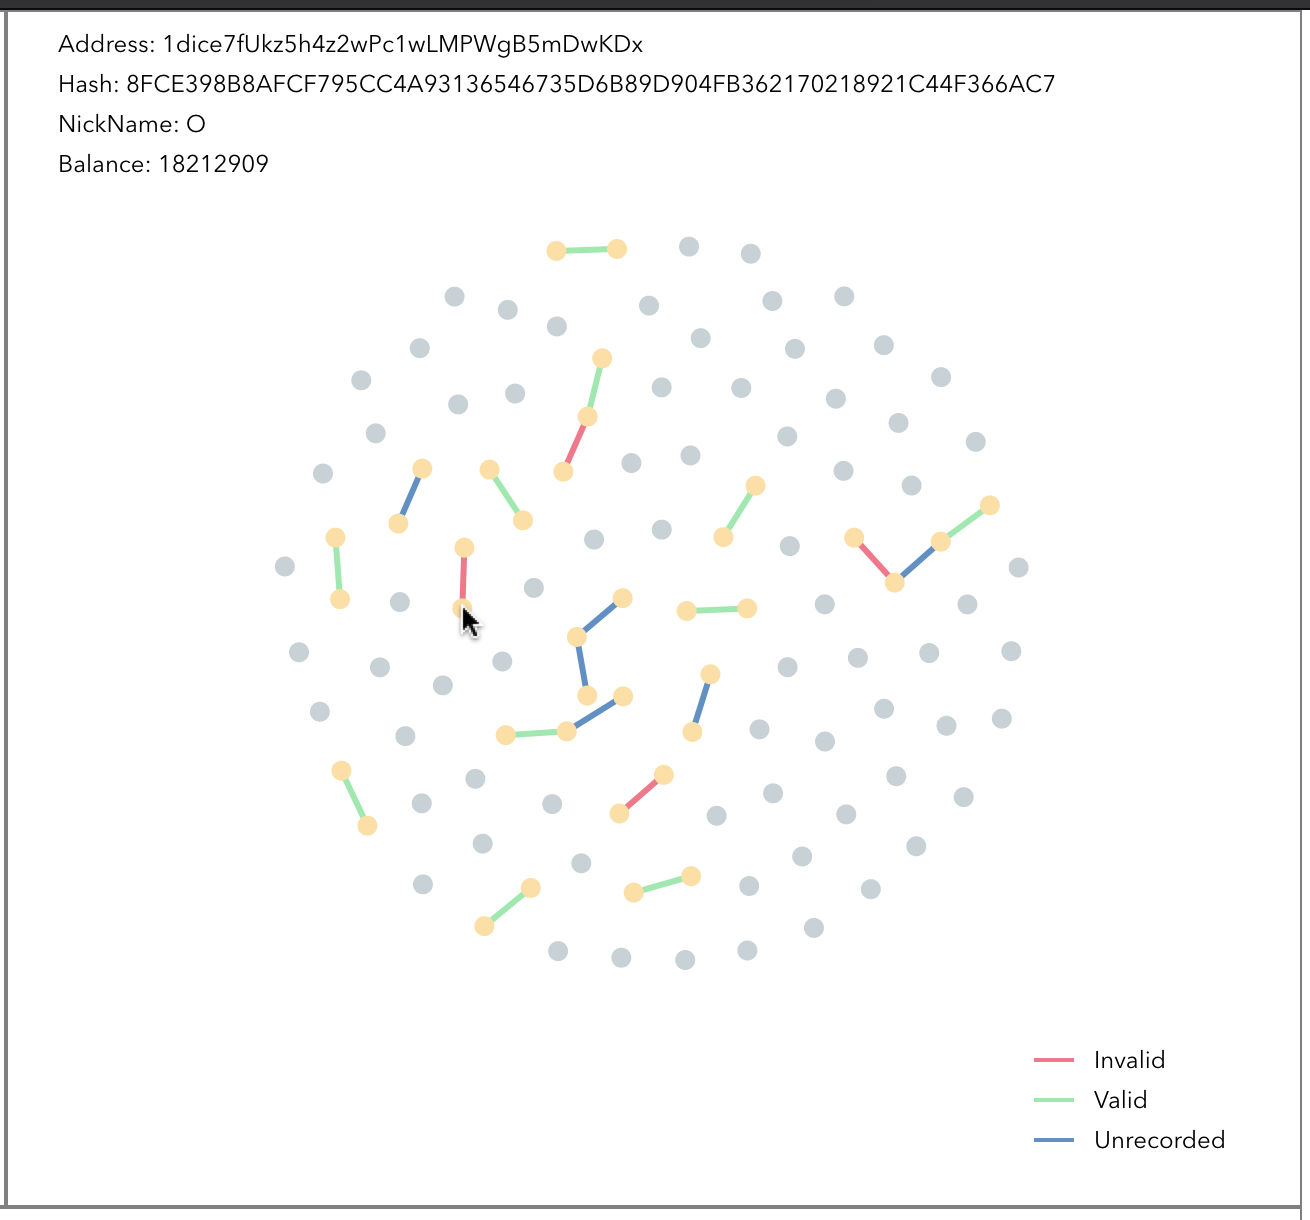
\includegraphics[width=\columnwidth]{transaction_hover.png}
		\caption{}
		\label{fig:transaction_hover}
		\end{center}
	\end{figure}

\subsection{Blocks}

\begin{figure}[!hbt]
		\begin{center}
		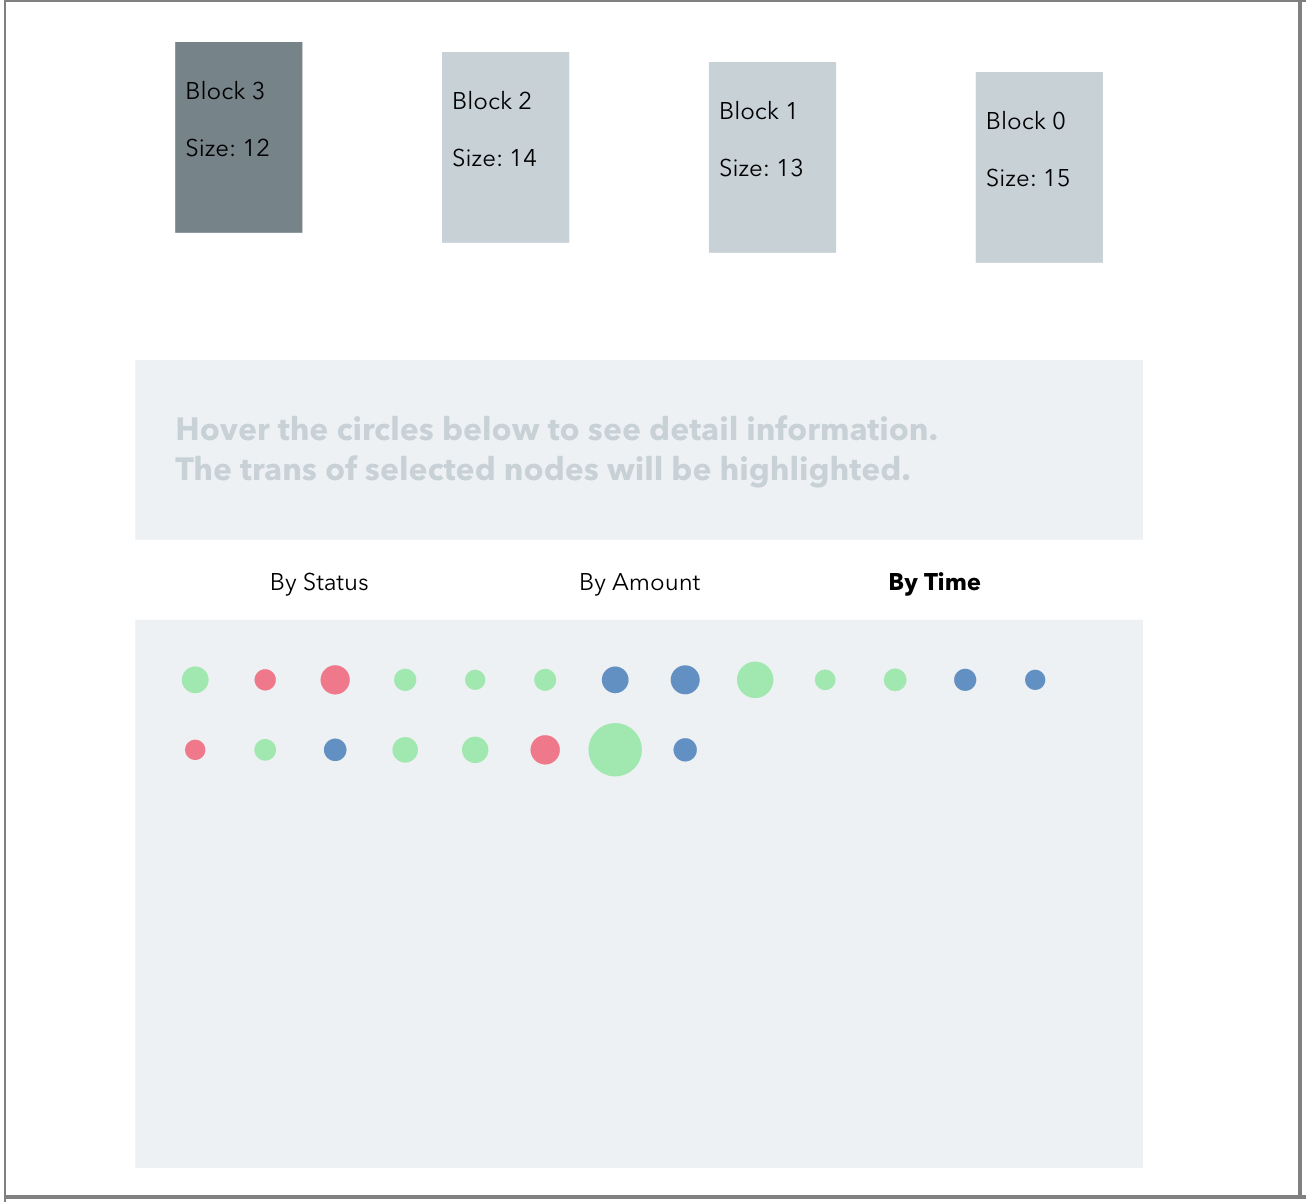
\includegraphics[width=\columnwidth]{blocks.png}
		\caption{}
		\label{fig:blocks}
		\end{center}
	\end{figure}
	
\begin{figure}[!hbt]
		\begin{center}
		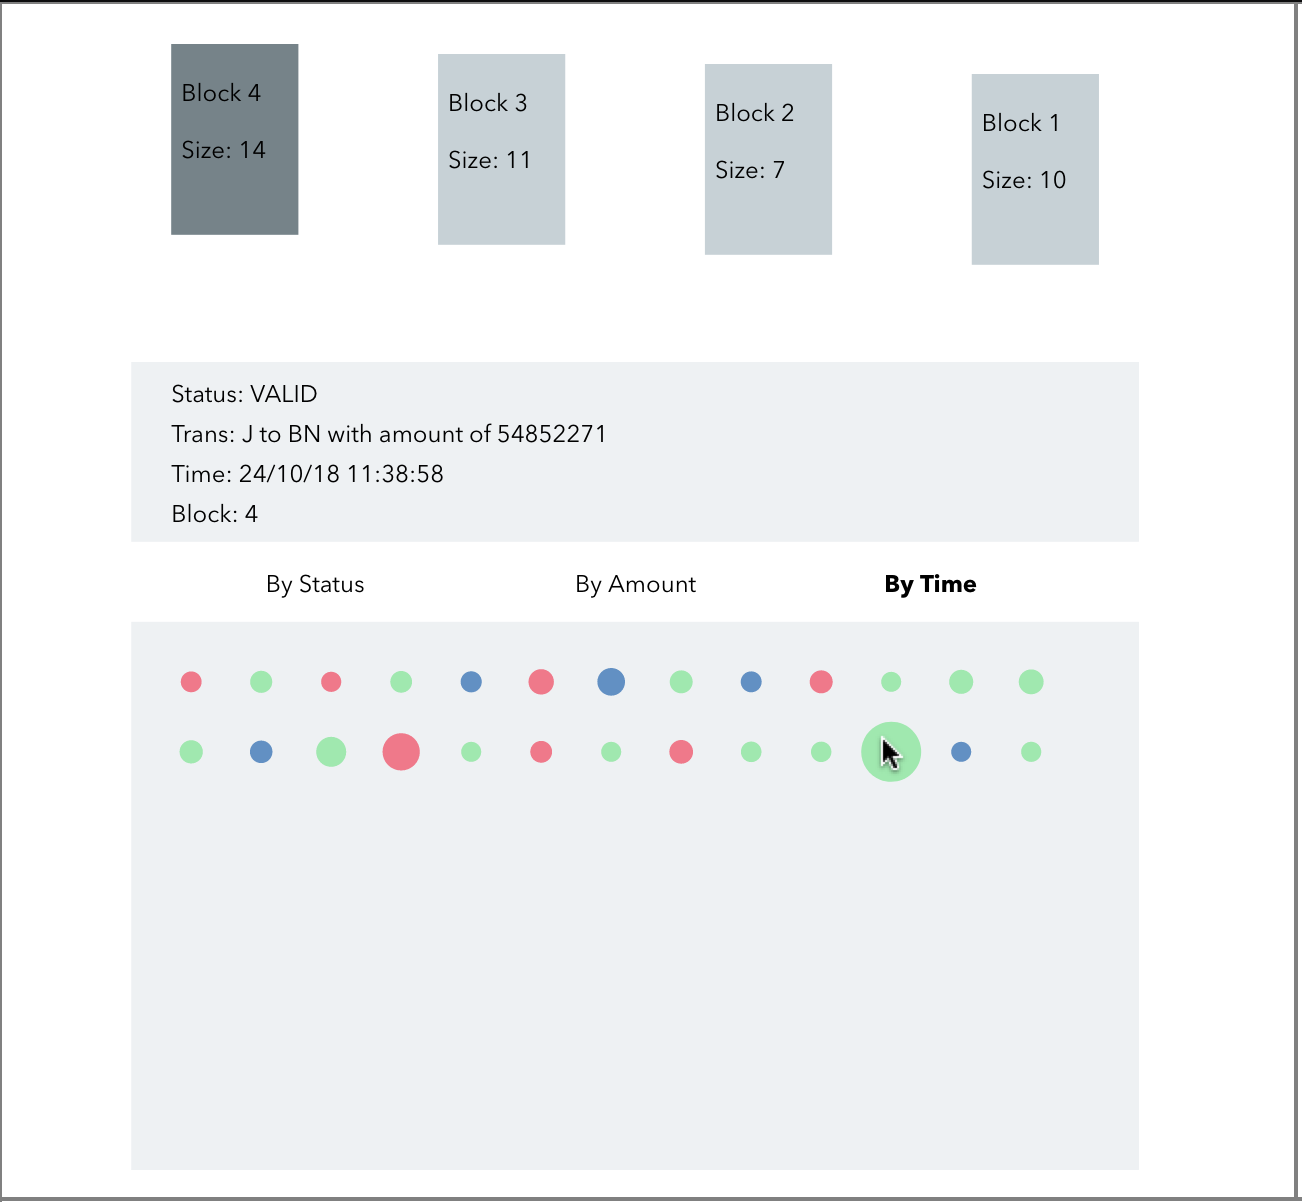
\includegraphics[width=\columnwidth]{block_hover.png}
		\caption{}
		\label{fig:block_hover}
		\end{center}
	\end{figure}
	
\section{Contributions}

\section{Conclusions}

\section{Future Directions}

\section{Team member attribution}

\begin{thebibliography}{5}

	%Each item starts with a \bibitem{reference} command and the details thereafter.
	\bibitem{HOP96} % Transaction paper
	J.~Hagenauer, E.~Offer, and L.~Papke. Iterative decoding of binary block
	and convolutional codes. {\em IEEE Trans. Inform. Theory},
	vol.~42, no.~2, pp.~429–-445, Mar. 1996.

\end{thebibliography}

% Your document ends here!
\end{document}